
\section{Pesquisa de Mercado} % (fold)
\label{sub:pesquisa_de_mercado}

	Atualmente, já existem outros robôs que também fazem limpeza automatizada. Para fins de pesquisa de mercado, foram encontrados os seguintes robôs \cite{techtudo}:

	\begin{itemize}
		\item \textbf{Aspirador de Pó Compacto Home UP:}

			O aspirador de pó inteligente tem um design compacto que permite entrar embaixo de sofás e camas, para remover a poeira. A opção tem armazenamento de até 400 ml com saco coletor e oferece escovas laterais. O aparelho funciona por bateria recarregável e está disponível na cor preto. A garantia do fornecedor é de 6 meses e ele tem dimensões de 400 x 345 x 135 mm, com peso de 2 Kg. O preço fica em torno de R\$ 819 em lojas online nacionais.

			\begin{figure}[H]
				\centering
				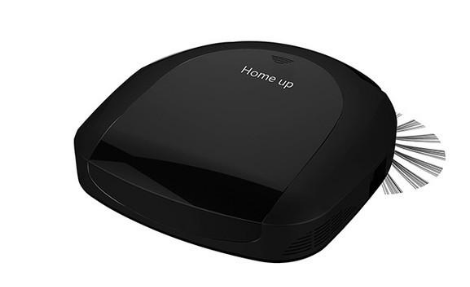
\includegraphics[scale=0.55]{figuras/pm_home_up.png}
				\caption{Aspirador de Pó Compacto Home UP.}
				\label{img:pm_home_up}
			\end{figure}

		\item \textbf{Aspirador de pó Ecovacs Beebot D35:}

			 O modelo da Ecovacs é equipado com sensores para evitar quedas ou bater em objetos, por exemplo. O aspirador de pó tem filtro bactericida e há uma bateria interna que dura cerca de 1 hora. É possível programar para fazer uma limpeza automática durante o dia e a garantia é de 1 ano. O design compacto permite entrar em espaços com 6 cm de altura e nas dimensões ele tem 300 x 290 x 50 mm, com peso de 2,2 kg. O aspirador robô pode ser comprado com preço a partir de R\$ 954.

			\begin{figure}[H]
				\centering
				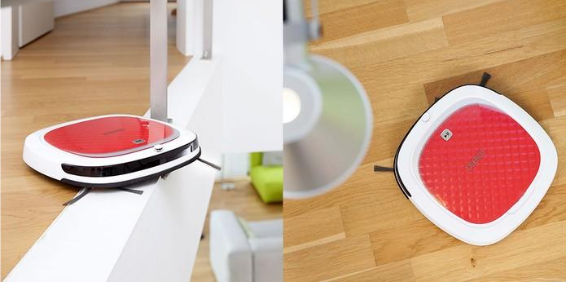
\includegraphics[scale=0.55]{figuras/pm_beebot_d35.png}
				\caption{Aspirador de pó Ecovacs Beebot D35.}
				\label{img:pm_beebot_d35}
			\end{figure}

		\item \textbf{Aspirador de pó robô Deboot 4:}

			Com uma configuração mais completa, o modelo Deboot 4 da Ecovacs tem função dupla de limpeza à vácuo e permite aspirar, varrer e até passar pano no piso da casa, com ações simultâneas. Por dentro está uma bateria recarregável e permite limpar embaixo os móveis ou nos cantos, com luzes indicadoras no painel. As funções programáveis permitem fazer limpezas automáticas, oferece sensores anti-choque e tem funcionamento por controle remoto. O preço é de R\$ 1.399 em lojas virtuais brasileiras.

			\begin{figure}[H]
				\centering
				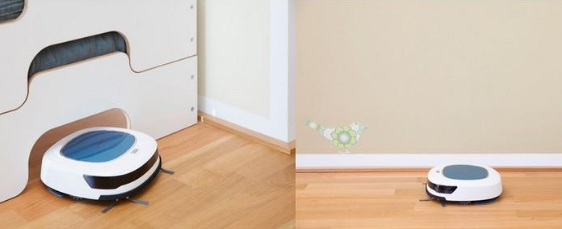
\includegraphics[scale=0.55]{figuras/pm_deboot_4.png}
				\caption{Aspirador de pó robô Deboot 4.}
				\label{img:pm_deboot_4}
			\end{figure}

	
		\item \textbf{Aspirador Roomba 620 iRobot:}

			O modelo iRobot da Roomba pemite ajustar funções smart e faz a limpeza em três etapas, de forma mais completa. A tecnologia AeroVac ajuda a recolher os resíduos durante o uso e a bateria dura cerca de 90 minutos. Estão disponíveis sensores para detectar poeira, o design tem laterais macias para não arranhar os móveis, além de identificar escadas. O aparelho pode ser usado em pisos de madeira, cerâmica e até carpetes. O tamanho é de 330,2 x 330,2 x 128 mm com peso de 3,6 kg e garantia de 12 meses. O preço fica em torno de R\$. 2.099 no Brasil, no modelo de cor branca.

			\begin{figure}[H]
				\centering
				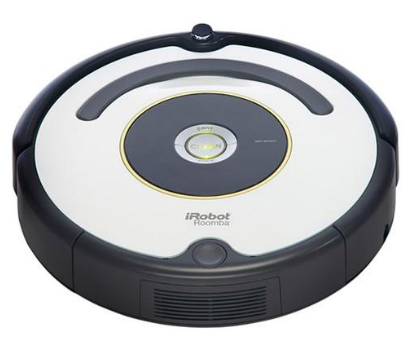
\includegraphics[scale=0.55]{figuras/pm_roomba.png}
				\caption{Aspirador Roomba 620 iRobot.}
				\label{img:pm_roomba}
			\end{figure}

	\end{itemize}

% subsection pesquisa_de_mercado (end)

